\documentclass{utue} %utue.cls required for Uni Tuebingen corporate design
\usepackage{amsmath}
\usepackage[hidelinks]{hyperref}
\def\sectionautorefname{Section}
% Values for title generation
\title{Cuda Implementation of Advanced Pencil Sketch Filter}
\author{Andreas Altergott, Raphael Braun, Stefan Burnicki}
\date{\today}

% Subtitle is optional. It represents what kind of work you did.
\subtitle{Practical course:\\Massive Parallel Programming SS2014}
\begin{document}

% You can place a teaser as follows. (Otherwise, just uncomment the following part)
\teaser{
    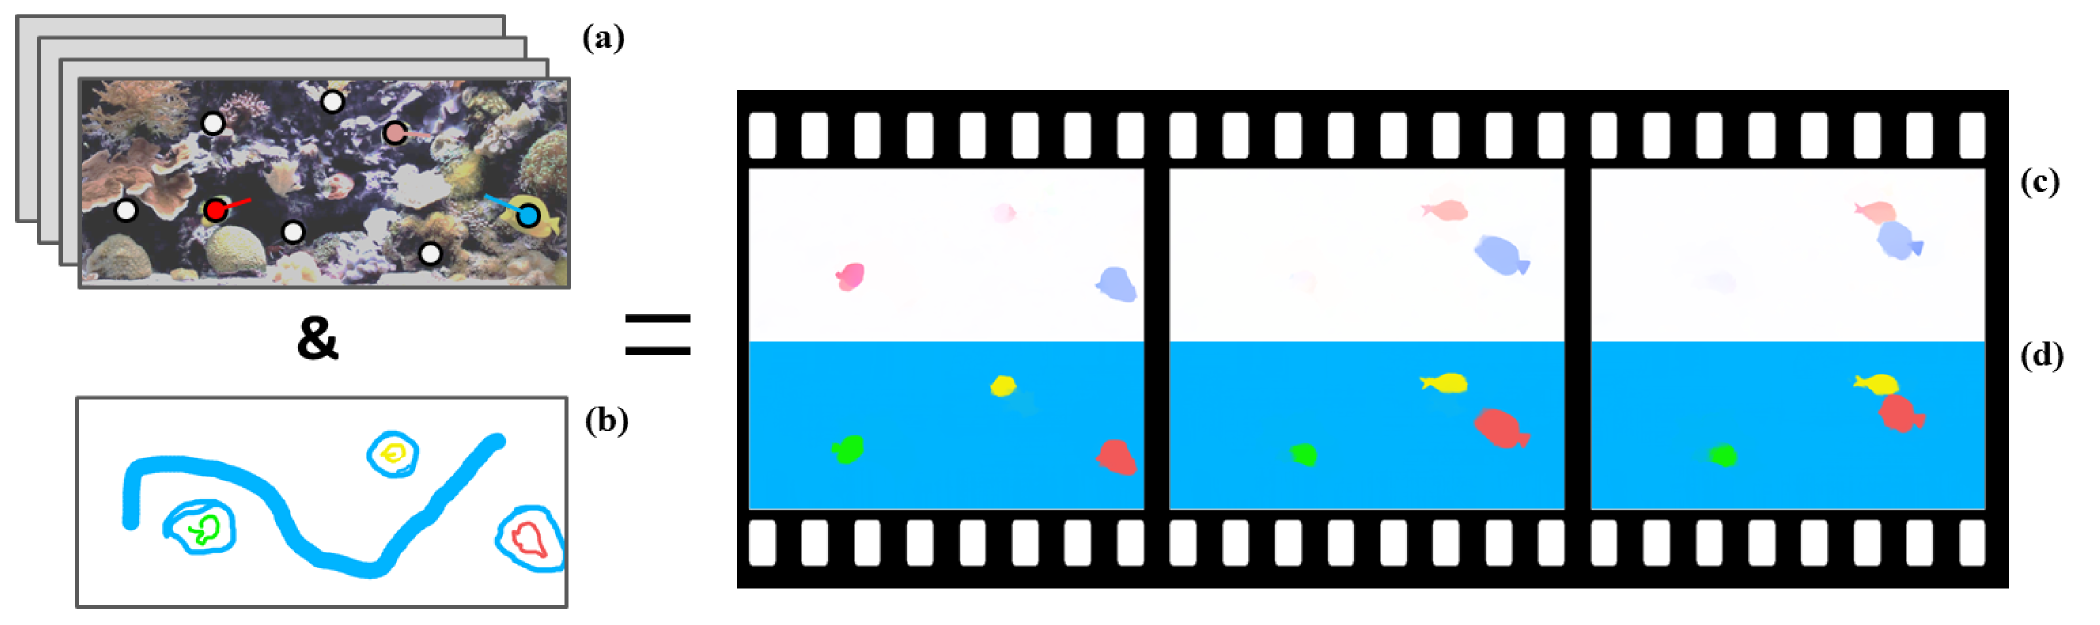
\includegraphics[width=.9\textwidth]{images/teaser.jpg}
    \caption{\label{fig:scribble}A application of the presented method is to
  consistently propagate user input scribbles through a video. Optical flow (c) is
calculated from the input video (a) using sparse feature matching. Then the
scribbles (b) are spread in space and time to generate (d)}
}     

% Creates title of document and additional title page.
\maketitle 
 
\section*{Abstract} 
This report is about blabla.

\section{Introduction}
Results of video manipulation application need to be consistent in time,
otherwise there will be visible temporal artifacts like flickering or any kind
of temporal noise. There are mathematical functions which can measure the
smoothness in arbitrary dimensions (smoothness in time is temporal consistency).
Such a function can be used as regularization term in optimizations. The method
that is presented in this report concentrates on graphics problems which can be
solved by minimizing a problem specific error function that consists of a data
term, which defines the problem, and a regularization term which enforces
consistency (see \autoref{eq:error-function}). 

The method introduced by the presented paper \cite{Lang:2012} efficiently
approximates the solution of the global optimization in
\autoref{eq:error-function}, thus it is generating practical temporal
consistency for long video sequences. This is done by exploiting well known
similarities between optimizations and nonlinear partial differential equations
(PEDs), which can be solved using anisotropic diffusion \cite{Weickert:1998}. As
anisotropic diffusion is closely related to edge aware filtering, efficient
image filtering is used to replace the optimization. More precisely, the data
term is separated from the regularization. The later is then approximated as an
efficient edge-aware filter on the first.

For this the domain-transform edge aware filter from
\cite{GastalOliveira2011DomainTransform} is used and extended such that can
simultaneously use and iteratively calculate optical flow vectors.

The proposed approach approximates the global optimization by introducing a
temporal smoothness assumption, resulting in high quality temporally consistent
results, with only very view and intuitive parameters which can be fixed for
each application. The method can be used for a whole class of image-based
graphic problems. Optical flow, disparity estimation and colorization are
popular instances of this problem class. The approach performs fast without
exploiting the massive parallelism of GPUs due to its simple and efficient
concept.

\autoref{method} gives a detailed description of the proposed method. This
ranges from the transformation of the expensive optimization to a simple
filtering step to a evaluation of the results including a short performance
comparison. In \autoref{applications} there is a brief list of applications
which were implemented by the authors using their new approach.

\section{Previous Work}
This section highlights the difficulty of solving the optimization problem in
\autoref{eq:error-function} by outlining other approaches and their
restrictions. The domain-transform paper
\cite{GastalOliveira2011DomainTransform} is left out on purpose, as it is
discussed in \autoref{domain-transform} in great detail.

The smoothness that is applied to a pixel by the regularization term depends on
the values of all the other pixels. Those dependencies often leads to non-convex
optimization problems, which are computationally infeasible for video volumes.

For this reason most existing methods which address the problem class in
\autoref{eq:error-function} concentrate on single-frame solutions, which are
computational tractable. However, single-frame solutions can not take account
for temporal consistency. Methods which also solve the temporal stability
problem typically use sliding windows to reduce computation costs
\cite{conf/psivt/HosniRBG11} and Kalman filtering to mix the results of
single-frame solutions \cite{conf/acivs/HoffkenOK11}. For those approaches it is
important to find the correct window size, as this parameter balances
computation costs and temporal smoothness. Poor parameter choices lead to
inconsistencies.

There also are methods which directly solve the global optimization using
precomputed optical flow as a representation of the frame-to-frame relations. An
example for this approach is \cite{Levin:2004:CUO:1015706.1015780}, which allows
to recolor a video based on sparse scribble input by the user. Those methods
generate high quality results but are computationally expensive and do not scale
well for higher resolution input images and videos.

\section{Method} \label{method} The problem class that is addressed by the paper
can be solved by minimizing error functions in the form:
\begin{equation}
  E(J) = E_{data}(J) + \lambda E_{smooth}(J)
  \label{eq:error-function}
\end{equation}
Where $J$ is the unknown solution, $E_{data}$ the application specific error
term and $E_{smooth}$ the regularization term which enforces neighborhood
smoothness.

Instead of solving this expensive optimization all at once, the data term is
calculated locally ($E(J)~=~E_{data}(J)$). The regularization term is replaced
by a edge aware filtering operation, which is then applied on $J$. This means
smoothness is created instead of solved for with a optimization.

To understand the mathematical justification for replacing a global optimization
by a local smoothing operation the method is explained for the calculation of
one single optical flow image as an example.

Given two consecutive images in a video $I_t$ and $I_{t+1}$, the pixel in the
unknown optical flow image $J(x,y)$ are motion vectors $\vec{\omega}(x,y) =
(u_{x,y}, v_{x,y})$ which describe the motion of pixel $(x,y)$ from $I_t$ to
$I_{t+1}$. The data term for the optical flow estimation is:
\begin{equation}
  E_{data}(u, v) = \sum_{(x, y)}\norm{I_t(x+ u, y + v) - I_{t+1}(x, y)}^{2}
  \label{eq:optical-flow-data}
\end{equation}
This means the color differences between the start pixels and the pixels to
which the motion vectors are pointing have to be as small as possible. The
regularization term is given as:
\begin{equation}
  E_{smooth}(u, v) = \sum_{(x,y)}(\norm{\nabla u_{x,y}}^2 + \norm{\nabla
    v_{x,y}}^2)
  \label{eq:optical-flow-smooth}
\end{equation}
$\nabla$ is the gradient magnitude operator, which measures
the change of a value at one position of the video volume. Little variations
results in small values (smooth), while big variations will create big values
(noise). So $E_{smooth}$ enforces smoothness to the flow by minimizes the total
quadratic variance of the flow gradient. 

By interpreting optical flow as a reaction-diffusion-system
\autoref{eq:optical-flow-smooth} can be considered the Dirichlet's energy of
$\vec{\omega}$. Minimizing it is equivalent to solving the Laplace equation
$-\Delta \vec{\omega} = 0$. The data term can be added to this minimization as
boundary condition. This yields a related heat equation, which is a special
differential equation with some initial conditions:
\begin{equation}
  \frac{\partial\vec{\omega}}{\partial t} = \alpha \Delta \vec{\omega}
  \label{eq:heat-equation}
\end{equation}
$\vec{\omega}$ is initialized as Dirac function based on the data term:
\begin{equation}
  \vec{\omega} = \begin{cases}
    J(x, y) & \text{if } \exists (x,y) \in J\\
    \vec{0} & \text{otherwise}
  \end{cases}
  \label{eq:initial-condition}
\end{equation}
The function which is the solution to this differential equation is the function
which has to be applied to $J$ (from the data term) to solves our optical flow
problem. In the isotropic case this function is known to be a Gaussian
convolution. However, images form a inhomogeneous medium and the solution to the
resulting nonlinear Partial Differential Equation is a anisotropic diffusion.
Please refer to \cite{Weickert:1998} for details in using anisotropic diffusion
for solving PDEs. \cite{paris2009bilateral} showed that anisotropic diffusion is
asymptotically equivalent to edge aware filtering, at least in the discrete
setting, which is good enough, as images are represented discretely.

That is why the regularization in \autoref{eq:optical-flow-smooth} can be
replaced by an edge-aware filtering on the correct input data $J$, which in the
case of optical flow can be calculated from \autoref{eq:optical-flow-data}.
The initialization of $J$ can be sparse as indicated in
\autoref{eq:initial-condition}. The authors of the presented paper exploit this
feature to calculate the initialization only for SIFT and Lucas-Kanade features.
It is very simple to find matches for such features in consecutive video frames
which results in efficient and reliable initial flow estimations.  The authors
use an out of the box implementation from the openCV library for this.  The only
thing that is left to do for the one-frame optical flow example is to specify
the used edge-aware filter.

\paragraph{Domain Transform} \label{domain-transform}
The domain transform edge aware filter from
\cite{GastalOliveira2011DomainTransform} is used and later extended for temporal
filtering. The edge awareness of a filter typically is based on filter weights
which change based on the image content. The domain transform works differently.
It transforms the distances between input pixels based on the image content,
such that a simple Gaussian filter on the transformed image yields an edge aware
result in the original domain. This transformation can only be done for 1D
signals.  However by applying the filter repeatedly to all rows (1D) and all
columns (1D) a full 2D Image can be filtered. The filtered solution after $N$
iterations is will be referred to as $J'$.
\autoref{fig:domain-transform-example} illustrates the transformation and
filtering process.

\begin{figure}[h!]
  \centering
  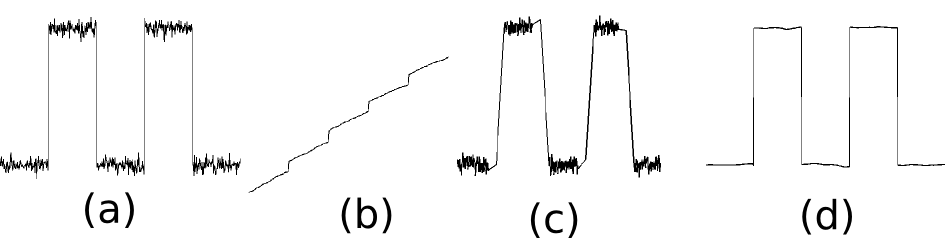
\includegraphics[width=.5\textwidth]{images/domain-transform.png}
  \caption{1D domain transform example. (a) Input signal, (b) transform
  of the sample distances, (c) Transformed signal, (d) Result of filtering (c) with
Gaussian filter and remap to original domain}
  \label{fig:domain-transform-example}
\end{figure}

A joined domain-transform filtering is used, meaning the domain transform is
calculated from the input image $I$. This transformation is then used to filter
$J$. Thus edge informations are obtained directly from the image $I$, not from
the flow estimate $J$.

The filter kernel (a sliding box filter) that is used in the domain transform
filter step is no interpolation filter, which is a problem if $J$ is sparsely
initialized.  Therefore the authors use a normalization image $G$. For pixels
$i$ in $J$, that were actually initialized, the corresponding pixel in $G$ are set
to one: $G_i = 1$.
Pixels that do not contain data in $J$ are set to 0. $G$ is filtered with the
exact same filter operation as $J$. The final result is computed as
$J''=\frac{J'}{G'}$.  \autoref{fig:joint-filter} shows the result of this joint
filtering operation on 1000 randomly chosen color values from a $250\times250$
image.

\begin{figure}[h!]
  \centering
  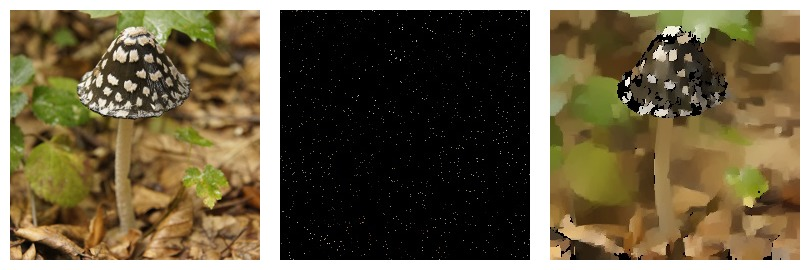
\includegraphics[width=0.5\textwidth]{images/joint-filter.jpg}
  \caption{Joint filtering. Left: Input image $I$ for domain transform; Center: Sparse
  color input $J$ generated by selecting 1000 random pixels from $I$, Right:
  Result of the joint filtering ($J''=\frac{J'}{G'}$)}
  \label{fig:joint-filter}
\end{figure}

\paragraph{Temporal Filtering} \label{temporal-filtering}
An additional filtering dimension is added to filter through time. As the domain
transform filter is separable and is already performing an $N$-step iteration
along $X$ and $Y$ direction, it is no problem to add another temporal dimension
$T$. One filter iteration will therefore consist of three filtering passes: a
pass in $X$ direction, in $Y$ direction and finally the result is filtered along
the motion path of the pixel through the video volume ($T$). An example for such
a motion path is shown in \autoref{fig:motion-path}. The pixels along the path
are filtered just like a regular row or column. Those paths are generated by
following the optical flow vectors in each frame, thus optical flow always has
to be calculated for the filtering regardless of the final application. 

\begin{figure}[htb]
  \centering
  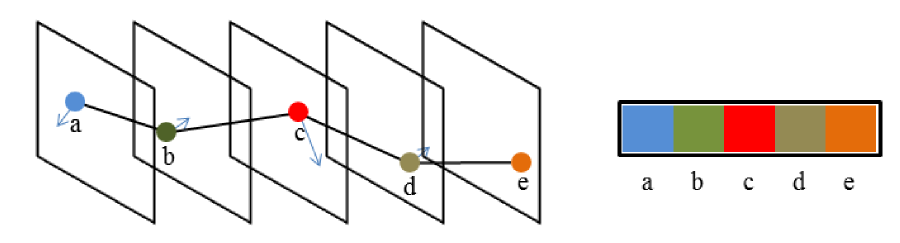
\includegraphics[width=0.5\textwidth]{images/paths.png}
  \caption{The motion path of one pixel. It is calculated by following the
  optical flow vectors (blue arrows). The temporal filter pass is applied to the
resulting 1D color vector (a,b,c,d,e)}
  \label{fig:motion-path}
\end{figure}

Requiring optical flow in order to calculate optical flow is a chicken egg
problem, which is solved by iteratively improving a rough estimation of the
flow. The first estimation is calculated using the sparse feature matching and
one spacial joint filtering step in $X$ and $Y$ direction. This initial guess is
then directly used for the first temporal pass $T$. The flow is then updated in
each of the N $X$-$Y$-$T$ iteration steps.


Three special cases have to be considered when filtering along a motion path:
\begin{enumerate}
  \item A path leaves the image boundaries
  \item Multiple paths point to one pixel
  \item No path from the previous frame is pointing to a pixel 
\end{enumerate}
Those cases are caught and handled such that each pixel in every frame belongs
to exactly one path: All pixels that do not belong to a path (due to 1. or 3)
are selected. New paths are created at the center of those pixels and
initialized by filtering backwards in time. In case 1. the path is ended and the
sliding box filter stops there. In case 2. one randomly chosen path is kept,
while the others are ended in the previous frame.

The filter sizes for the spacial passes ($\sigma_s, \sigma_r$) and for the
temporal pass ($\sigma_{st}, \sigma_{rt}$) can be controlled separately.

\paragraph{Confidence} \label{confidence}
Thanks to the normalization image $G$ it is very simple to add confidence values
$\beta_i$ to the initial data $J_i$, where $i$ is a pixel in a frame.
Differences of matched feature descriptors can be used as confidence values for
the optical flow and disparity estimation. The better the matches the higher the
confidence. The confidence is directly written into the normalization image $G_i
= \beta_i$ and multiplied to the data image $J$ by a per element multiplication
$J \cdot G$.  The result is then calculated the same way as before: $J'' =
\frac{(G\cdot J)'}{G'}$. \autoref{fig:confidence} illustrates the effect of the
confidence values.

\begin{figure}[htb]
  \centering
  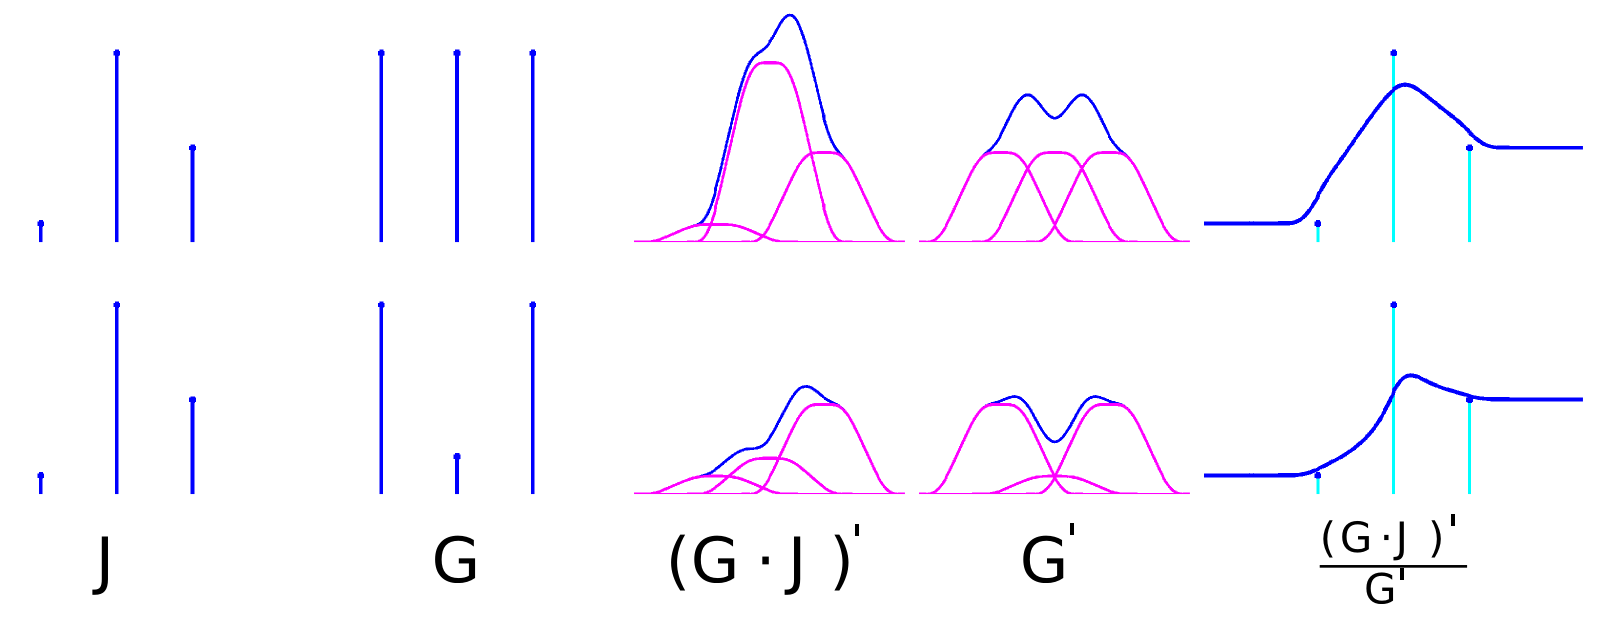
\includegraphics[width=0.5\textwidth]{images/confidence.png}
  \caption{Demonstration of the confidence values applied to a 1D signal. In the
    top row all samples have the same confidence. In the bottom row the
    confidence of the middle sample is reduced. The
    purple line shows the contribution of a point.}
  \label{fig:confidence}
\end{figure}

\paragraph{Iterative Occlusion Estimates} \label{iterative-occlusion-estimates}
An occlusion estimate is added, which lowers the confidence in regions where
the flow estimations prove to be unreliable. This automatically emphasizes
reliable estimations. The reliability of a flow vector is estimated by
computing both forward and backward flow vectors ($\vec{\omega^f}$ and
$\vec{\omega^b}$) in each frame and applying a penalty function $\rho$ to the
sum of those vectors. As they point in different directions, their sum should
be 0:
\begin{equation}
  \rho = \left(1-\abs{\vec{\omega^f} + \vec{\omega^b}}\right)^{\theta}
  \label{eq:penalty}
\end{equation}
$\theta$ defines the shape of the curve and was set to 5 for all applications
(see \autoref{fig:penalty-shape}).
The penalty has to be updated in each iteration as the flow changes. In the
$n$th iteration $G^n$ is updated with $G^n~=~G^{n-1}~\cdot~p^{n-1}$. $J^n$ is
updated the same way: $J^n~=~J^{n-1}~\cdot~p^{n-1}$.

\begin{figure}[htb]
  \centering
  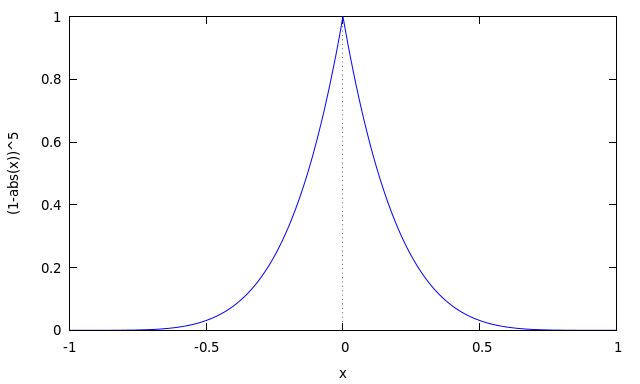
\includegraphics[width=0.35\textwidth]{images/penalty.png}
  \caption{Shape of the penalty function for $\theta = 5$.}
  \label{fig:penalty-shape}
\end{figure}

\subsection{Evaluation} \label{evaluation}
\autoref{fig:improvements} shows the improvements that are gained by the
described methods. The first two rows are optical flow vectors and the last a
scribble propagation. The first column shows the result when the temporal
dimension is naively filtered straight through the video volume. For the second
volume motion paths were followed. The last two columns show the effect of
confidence and occlusion estimation. Note that especially the edge regions are
improved.

\begin{figure}[htb]
  \centering
  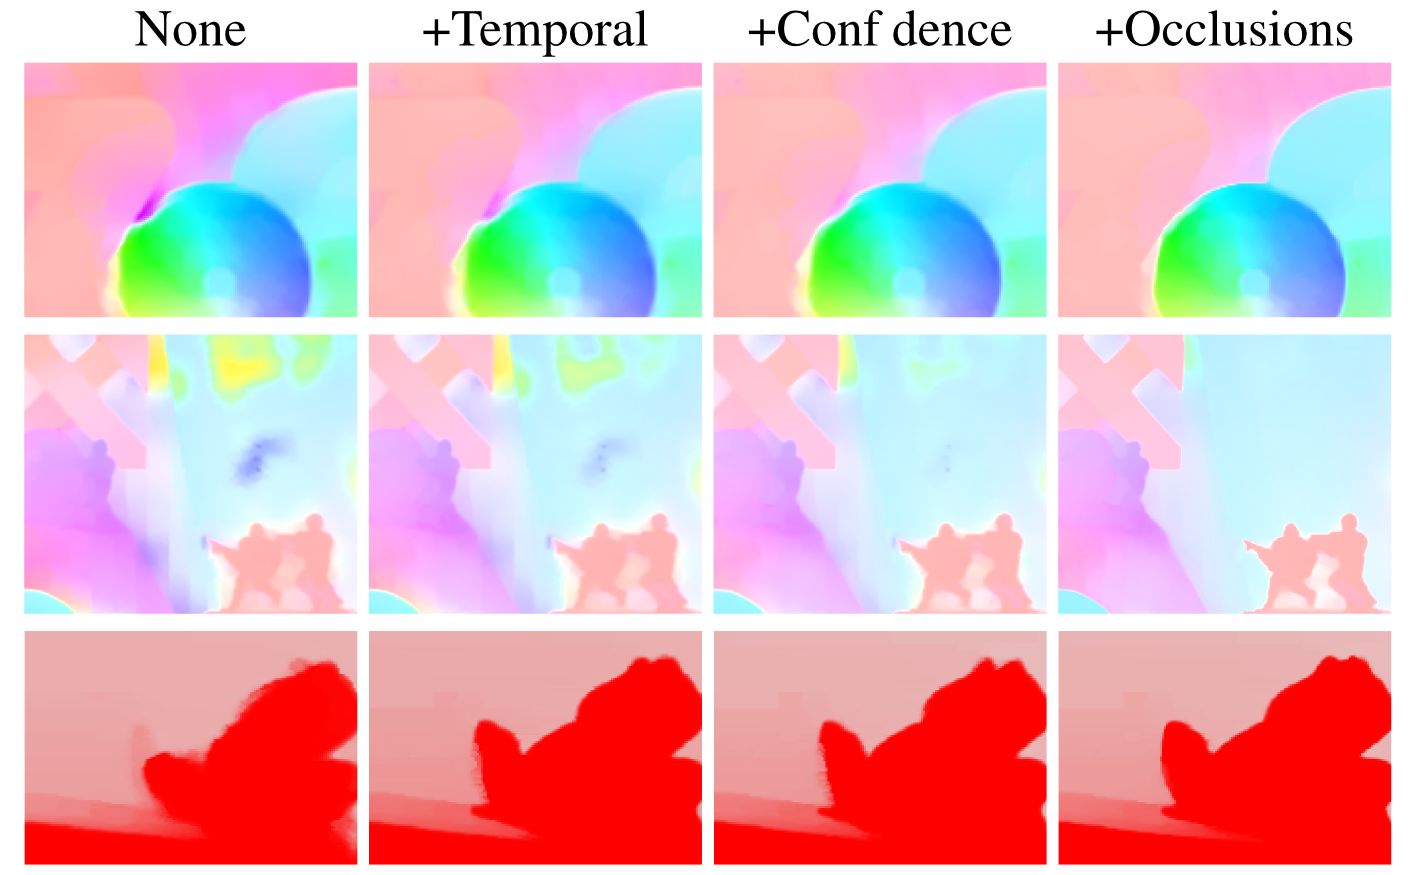
\includegraphics[width=0.5\textwidth]{images/improvements.png}
  \caption{The effect of each processing step: temporal filtering, confidence
  and iterative occlusion estimates. The first two rows show color coded optical flow
vector estimations, the last row is a scribble propagation which dyes a frog to be red.}
  \label{fig:improvements}
\end{figure}

There is no ground truth data available for long temporal optical flow
computations, therefore a qualitative validation is not really possible. However
the comparisons in the supplemental video to other state of the art methods
suggest that this new method is superior to all other methods in respect to
correctness and consistency.

The fact that a descriptor based feature matcher is used for the initial sparse
optical flow calculation enables this method to correctly track small, fast
moving object, as long as they have matchable features. Other optical flow
calculation approaches use windows to reduce computation cost and scale-space
pyramids for large motions, so fast moving objects are detected in downscaled
images. Therefore small fast moving objects disappear completely.

\autoref{tab:performance} shows a performance comparison of the presented
approach to some state of the art optical flow calculation approaches.
\begin{table}[htb]
  \centering
  {\footnotesize
  \begin{tabular}{|c|cc|}
    \hline
    Method & Time per output frame & Total for 8 frames\\
    \hline \hline
    \cite{Rhemann:2011:FCF:2191740.2191908} & 55 seconds & 7.3 minutes\\
    \cite{Zimmer:2011:OFH:1969654.1969711} & 620 seconds & 1.4 hours\\
    \cite{conf/iccv/VolzBVZ11} & 40 minutes & 5.4 hours\\
    presented& 625 ms & 5 seconds\\ \hline
  \end{tabular}}
  \caption{Performance comparison for the optical flow calculation to different
  approaches on the same 8 frame sequence ($640\times640$ resolution)}
  \label{tab:performance}
\end{table}

\section{Applications} \label{applications}
The temporal consistency that can be achieved using the described method is
usable for many applications, however as the optical flow is always needed for
temporal filtering it is calculated no matter which application is implemented.
Optical flow by itself can be used used for various applications like frame
interpolation, motion blur or motion magnification
\cite{journals/tog/LiuTFDA05}.

\paragraph{Disparity Estimation} \label{disparity-estimation}
Disparity estimation is about computing the correspondence between a pair of
stereoscopic images. The result $J_{xy}=d_{xy}$ can be used as depth map for
various tasks. Finding correspondences in stereoscopic images is very similar to
calculating optical flow from consecutive video frames:
\begin{align*}
  E_{data}(d) &= \sum_{(x,y)}\norm{I^r(x + d_{xy}, y) - I^l(x,y)}^2\\
  E_{smooth}(d) &= \sum_{(x,y)}\left( \norm{\nabla d_{xy}} \right)^2
\end{align*}
$J$ is sparsely initialized by feature matches between $I^r$ and $I^l$ and then
filtered as it was done for optical flow. \autoref{fig:disparity} shows an
example.
\begin{figure}[htb]
  \centering
  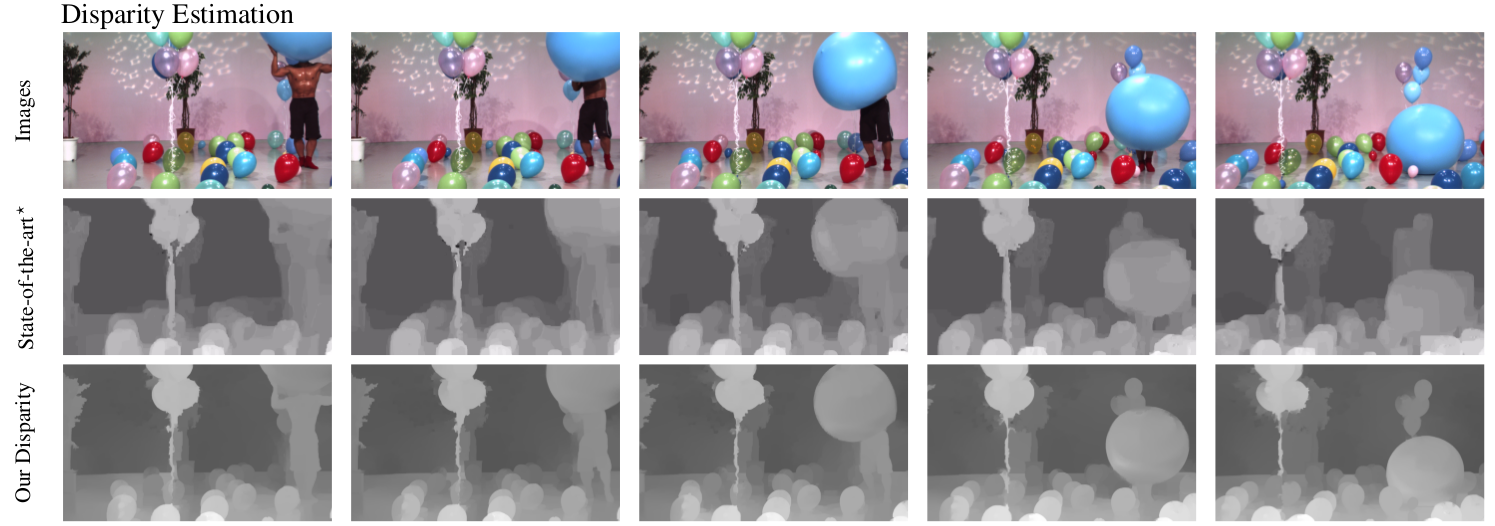
\includegraphics[width=0.5\textwidth]{images/disparity.png}
  \caption{The results of the disparity estimation is compared of a state of the
  art dataset provided by the MPEG group for testing. Again the results of the
proposed method is more stable in time. Less holes are randomly appearing and
disappearing compared to MPEG data set.}
  \label{fig:disparity}
\end{figure}

\paragraph{Colorization and Scribble Propagation} \label{colorization}
The approach can be used to propagate user input (pen strokes) through a given
video. The scribbles can have arbitrary meaning like color input for
colorization or ids for object labeling. The input scribbles $s_j$ from frame
$j$ are used to initialize $J_j = s_j$. Then the joint temporal smoothing is
applied to create intermediate frames. In average only every 20th frame needs
own scribble data.  \autoref{fig:scribble} shows an example for this
application.

\paragraph{Depth up-sampling} \label{up-sampling}
Depth sensor data from devices like Microsoft Kinects often suffer from bad
resolution, temporal noise and holes. The authors use their technique to filter
this data ($J$) using the image data from the Kinects camera for the domain
transform. As a result $J'$ is getting up-sampled, holes are getting filled and
noise is smoothed. \autoref{fig:depth-upsampling} shows a before-after
comparison.
\begin{figure}[htb]
  \centering
  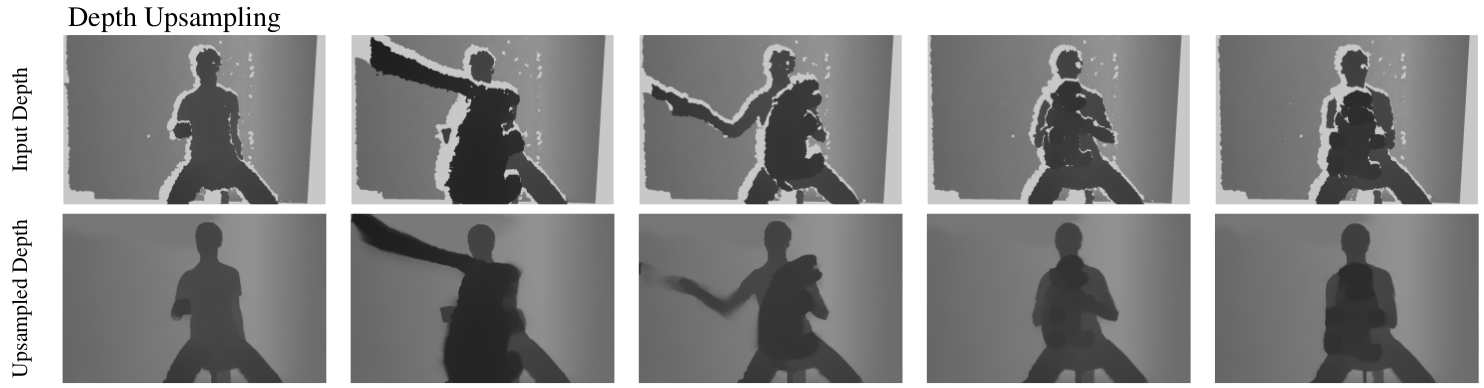
\includegraphics[width=0.5\textwidth]{images/depth.png}
  \caption{Low resolution and extremely noisy depth maps from a Microsoft Kinect
  is up-sampled and filled (white holes) using the same joint filtering
operation as it is used for the optical flow calculation. The image data from
the Kinect camera is used for the domain transform.}
  \label{fig:depth-upsampling}
\end{figure}

\paragraph{Saliency} \label{saliency}
Visual saliency maps are used in many graphics applications as they highlight
important regions in images. They can be used to change the aspect ratio of a
video without distorting important features (persons). In this case temporal
inconsistencies show up as wobbling. The authors used a per frame saliency
calculation $l$ as initialization for $J(x,y) = l(x,y)$ and applied the temporal
smoothness operation to gain consistent results. \autoref{fig:saliency} shows
the difference between the unfiltered and the filtered saliency.
\begin{figure}[htb]
  \centering
  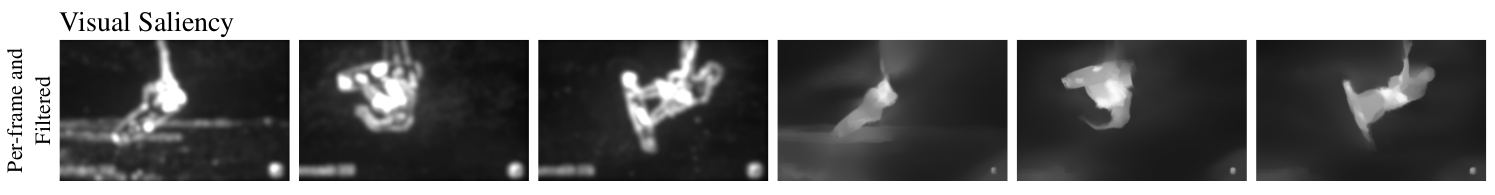
\includegraphics[width=0.5\textwidth]{images/saliency.png}
  \caption{First three images show the per frame saliency calculation, which are
  then temporally filtered to create the smooth results on the right.}
  \label{fig:saliency}
\end{figure}

\section{Conclusion}
A simple and efficient approach was presented that simplifies difficult global
optimization problems like optical flow and disparity calculations using
temporal edge aware filtering. The method creates temporal consistent results
for many image based graphics problems. Sparse feature matches can be used as
input for the joint filtering operation to replace costly global minimizations.

There are some limitations to the approach. It is possible that objects are not
detected if they do not provide enough features to match. This issue can be
addressed by adapting the parameters of the feature matcher to find as many
features as possible. The effect of faulty features is minimal as their
confidence is low, so they are filtered out.

As the method relies on edge preserving filtering problems occur if important
object boundaries are not well defined in the input images. Unwanted bleeding
artifacts can show up on such edges. Special care must be taken in the scribble
propagation application to place the input scribbles close to edges, as object
boundaries could otherwise be missed which causes unwanted color bleedings. A
true global solution does not suffer from this problem. The authors suggested an
extension that could fix this issue.

For me as writer of this report the described method in the paper was quite easy
to comprehend and written in enough detail for a full reimplementation.

\bibliographystyle{alpha}
\bibliography{bibliography}


\end{document}

